% !TEX root = ../Main.tex
\documentclass[../Main.tex]{subfiles}
\begin{document}

Das OpenStack Projekt Nova (Compute) ist für die Provisionierung von virtuellen Instanzen zuständig.
Dabei sind die Dienste \textbf{Keystone}, \textbf{Glance}, \textbf{Neutron} und \textbf{Placement} erforderlich
mit denen Nova interagiert \citep{NovaDocs}.

\begin{figure}[h]
    \centering
    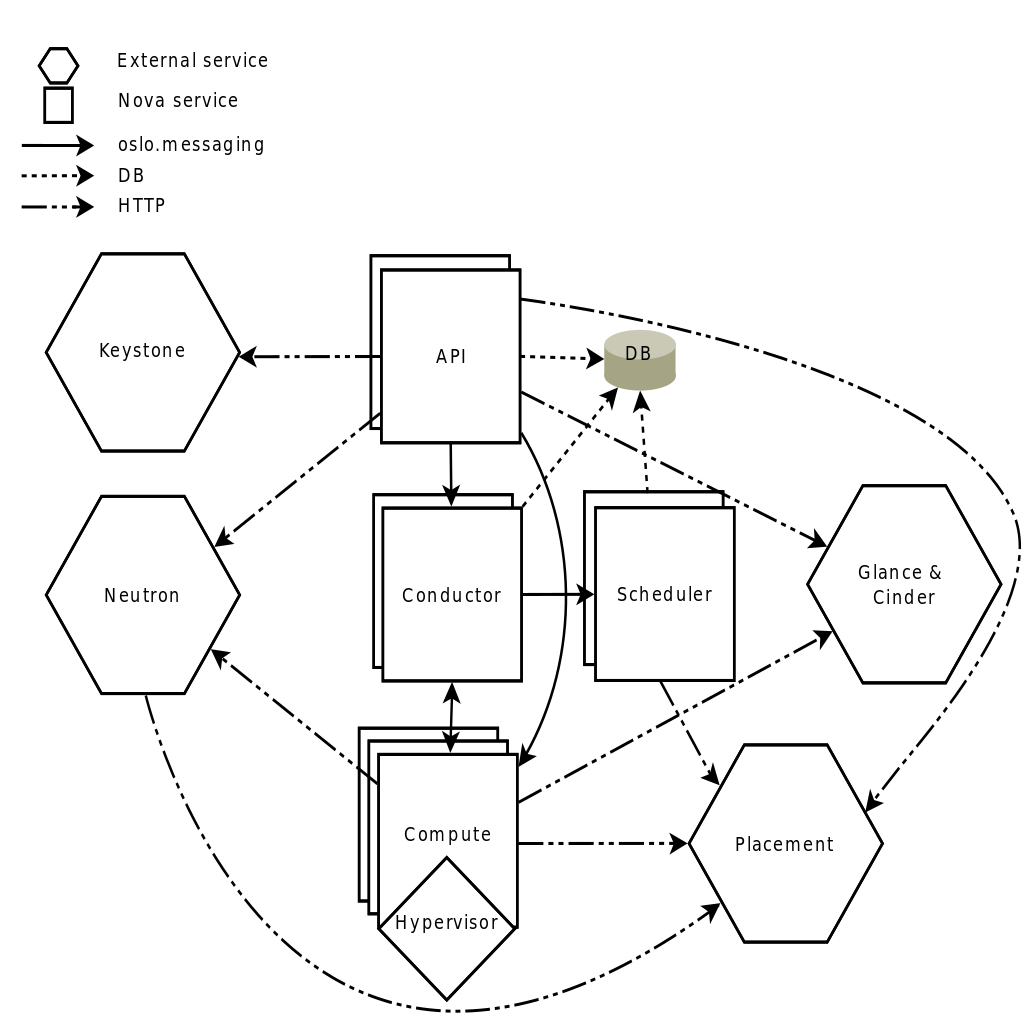
\includegraphics[width=0.9\columnwidth]{Images/NovaSystemArchitecture.png}
    \caption{Nova System Architektur \citep{NovaSystemArchitecture}}
\end{figure}

Neue Instanzen können dabei über die Nova API erstellt werden. Über eine Message Queue wird die
\textbf{Request Specification} dann an den Nova Conductor gesendet. Dieser koordiniert die einzelnen
Aufgaben und agiert als Datenbank Proxy \citep{NovaSystemArchitecture}.
Der Scheduler ist dabei für die Entscheidung zuständig auf welcher Compute Node eine Instanz
allokiert werden kann und welche Node dafür am besten geeignet ist. Der Placement Dienst allokiert
dabei die Ressourcen und bekommt von den Compute Nodes Informationen über die aktuelle Hardwarespezifikation (Traits)
und Auslastung (Resources).

\subsection{Nova Scheduler}

Nova Scheduler implementiert den \textbf{Filter Scheduler}, der die Hosts anhand von Eigenschaften filtert
und gewichtet \citep{ComputeSchedulers}.
\begin{figure}[h]
    \centering
    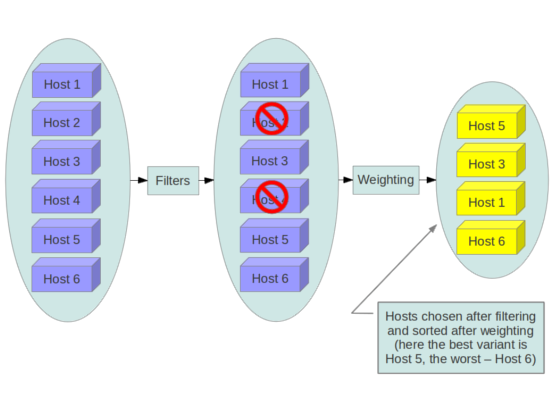
\includegraphics[width=0.9\columnwidth]{Images/NovaFilterWorkflow.png}
    \caption{Nova Filter Workflow \citep{ComputeSchedulers}}
\end{figure}

\subsubsection{Filter}

In einem ersten Schritt wird geprüft welche Hosts den Anforderungen
genügen. Alle konfigurierten \textbf{Filter} müssen dabei den Host akzeptieren \citep{ComputeSchedulers}.

Sei $F$ die Menge aller Filter, dann muss gelten:

\begin{center}
    $\forall f \in F: f(Host, RequestSpec) = True$
\end{center}

Andernfalls wird der Host nicht weiter
für das Scheduling der Instanz betrachtet.

\subsubsection{Weigher}
\label{chapter:Weigher}

Danach werden die akzeptierten Hosts mit sogenannten \textbf{Weigher} gewichtet und sortiert.

Das Gewicht eines Hosts berechnet sich aus \citep{NormalizedWeights}:
\begin{center}
    $weight = m_1 * norm(w_1) + m_2 * norm(w_2) + ...$
\end{center}
Dabei ist $w_i$ das Gewicht und $m_i$ der Multiplikator des \textbf{Weigher} $i$. Das Gewicht
$w_i$ wird zwischen $0$ und $1$ normalisiert. Über den Multiplikator lässt sich der Einfluss
bestimmter \textbf{Weigher} ändern. Ist $w_i = 0$ oder $m_i= 0$, dann nimmt der Weigher keinen Einfluss
auf die Gewichtung.

\begin{figure}[h]
    \centering
    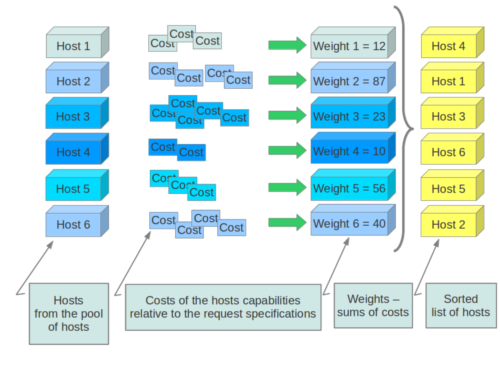
\includegraphics[width=0.9\columnwidth]{Images/nova-weighting-hosts.png}
    \caption{Nova Weighting Hosts \citep{ComputeSchedulers}}
\end{figure}

\subsubsection{Placement}
\label{chapter:PlacementAPI}

Nach erfolgter Gewichtung versucht der Nova Scheduler die Ressourcen des \textbf{Request Spec} auf dem Host mit
dem höchsten Gewicht zu allokieren. Die einzelnen Ressource-Typen werden dabei als sogenannte \textbf{Classes} verwaltet \citep{PlacementDocs}.
Dies sind zum Beispiel \textbf{VCPU}, \textbf{{MEMORY\_MB}} und \textbf{{DISK\_GB}}. Erst wenn diese
Allokation erfolgreich ist, wird die Instanz auf dem Host erstellt. Schlägt die Allokation oder Erstellung, sogenanntes \textbf{Spawning}, fehl wird versucht
die Instanz auf dem Host mit dem nächstkleineren Gewicht zu erstellen.

\subsubsection{Metadata und Extra Specs}

Nova bietet zusätzlich die Möglichkeit Metadaten an Hosts oder sogenannte Extra Specs an Flavor zu setzen. Ein Flavor definiert
dabei eine bestimmte Hardwarekonfiguration einer Instanz \citep{FlavorDocs}. Die Daten werden dann vom Nova Scheduler
oder eigenen Filter und Weigher genutzt. Der Extra Spec \textbf{quota:vif\_outbound\_peak=65536} beschränkt zum Beispiel die maximale ausgehende Netzwerk-Übertragungsrate auf 512 Mbit/s.

\subsubsection{Erweiterung des Nova Schedulers}

Im Beispiel ist ein Filter implementiert, der es nur erlaubt eine einzelne Instanz
pro \textbf{Request Spec} zu erstellen.

\begin{minted}[bgcolor=LightGray]
{python}
from nova.objects.request_spec import RequestSpec
from nova.scheduler.host_manager import HostState
from nova.scheduler import filters

class SingleInstancePerRequestFilter(filters.BaseHostFilter):
    RUN_ON_REBUILD = False

    def host_passes(
        self, host_state: HostState, request_spec: RequestSpec
    ):
        # Only allow user to schedule a single instance at a time
        return request_spec.num_instances == 1
\end{minted}

Eine Implementierung eines Weighers der einen Host anhand seiner Instanzen gewichtet
wird im folgenden Beschrieben.
Dadurch werden Hosts mit mehr Instanzen priorisiert (Stacking).
Über die Metadata der Host Aggregates (instance\_count\_weight\_multiplier) kann dann die Wichtigkeit
des Weighers bestimmt werden. Ein Aggregate ist dabei eine Gruppierung von Hosts
die gemeinsame Eigenschaften besitzen. Ein negatives Gewicht führt zu einem
Spreading, daher die Instanzen werden möglichst breit auf den Hosts verteilt.

\begin{minted}[bgcolor=LightGray]
{python}
from nova.scheduler import weights
from nova.scheduler.host_manager import HostState
from nova.objects.request_spec import RequestSpec

class InstanceCountWeigher(weights.BaseHostWeigher):
    def weight_multiplier(self, host_state: HostState):
        """Override the weight multiplier."""
        return utils.get_weight_multiplier(
            host_state, 'instance_count_weight_multiplier',
            1.0)

    def _weigh_object(
        self, host_state: HostState, request_spec: RequestSpec
    ):
        return host_state.num_instances # Stack based on Instances
\end{minted}

Darüber hinaus kann ebenfalls im Filter und Weigher auf Metadata und Extra Specs zugegriffen werden.
Ein Zugriff auf den Extra Spec \textbf{customscope:someattribute} ist beispielsweise so möglich:

\begin{minted}[bgcolor=LightGray]
{python}
value = request_spec.flavor.extra_specs.get('customscope:someattribute')
\end{minted}

Seit dem OpenStack Release Ussuri und der Compute API Version 2.86 unterstützt Nova
die Validierung von Flavor Extra Specs \citep{ExtraSpecsValidation}. Horizon nutzt aktuell
eine ältere Version der API, weshalb dort die Validierung nicht erfolgt. Die Validierung muss
aktiv vom Client angefordert werden, in dem eine entsprechende API Version genutzt wird. Mit
der OpenStack CLI ist das beispielsweise wie folgt möglich:

\begin{minted}[bgcolor=LightGray]
{shell}
openstack --os-compute-api-version 2.86 flavor set \
--property customattribute:someattribute=optionA $FLAVOR
\end{minted}

Für die Validierung von eigenen Scopes und Attributen kann ein
Validator implementiert werden \citep{ComputeSchedulers}. Dieser muss unter
dem Python Entrypoint \textbf{nova.api.extra\_spec\_validator} registriert werden und für
den Dienst Nova API sichtbar sein.


\begin{minted}[bgcolor=LightGray]
{python}
from nova.api.validation.extra_specs import base

def register():
    validators = [
        base.ExtraSpecValidator(
            name='customscope:someattribute',
            description='Custom Enum Attribute',
            value={
                'type': str,
                'enum': [
                   'optionA',
                   'optionB'
                ]
            }
        ),
    ]

    return validators
\end{minted}

\biblio % Needed for referencing to working when compiling individual subfiles - Do not remove
\end{document}
